\documentclass{beamer}
\usepackage{graphicx}
\usepackage{subcaption}
\usepackage{multirow}
\usepackage{booktabs}
\usepackage{pdfpages} 
 %\usepackage{beamerthemesplit} %// Activate for custom appearance

\title{Project for 2012 Argonne-Chicago Initiative for Computational Economics.}
\author{Anmol Bhandari\\
	     Alessandro Graniero \\
		Luis Quintero \\
		Phillip Renner
}
%\date{\today}
\date{07/20/2012}



\begin{document}

\frame{\titlepage}


\frame
{
  \frametitle{ The risk-free rate in heterogeneous-agent incomplete-insurance economies. Hugget (1993).}
Motivation of paper
\begin{itemize}
	\item Motivation of the paper:
	\begin{itemize}
		\item  calibrated representative agent economies do not match the real return to equity and 
		risk free debt. In particular they predict a risk free rate that is too great. Market imperfections can help explain this. 
		\item The paper looks at idiosyncratic shocks and incomplete insurance: credit balance with a central credit authority 
		must remain above a  fixed credit limit $\underline{a}$.
	\end{itemize}
	\item Our  contribution: 
	\begin{itemize}
		\item Hugget's computation of the model uses a discrete grid for the state space. We will use projection methods with 
		continuous Chebysev polynomials for the policy functions and the stationary distribution. Also, we will use shape 
		preserving constraints to guarantee some desired features of the stationary distribution.
	\end{itemize}
\end{itemize}
}

\frame
{
  \frametitle{  The risk-free rate in heterogeneous-agent incomplete-insurance economies. Hugget (1993).}
  Setup 
\begin{itemize}
	\item Preferences: 
		\begin{eqnarray*}
		E \left [ \sum_{t=0}^\infty \beta^t u(c_t) \right ] & where & \beta \in (0,1)\\
		u(c) = \frac{c^{1-\sigma}}{1-\sigma}
	\end{eqnarray*}
	\item Technology:
	\begin{itemize}
			\item Perishable endowment shocks $S=\{s_h,s_l\}$ that follow a markov process with 
			stationary transition probability $p(s' \vert s) >0$.
	\end{itemize}
	\item Markets:
	\begin{itemize}
		\item  Credit balance with a central credit authority must remain above a  fixed credit limit $\underline{a}$.
	\end{itemize}

\end{itemize}
}

\frame
{
  \frametitle{  The risk-free rate in heterogeneous-agent incomplete-insurance economies. Hugget (1993).}
  Agents Problem 
\begin{itemize}
	\item Bellman Equation: 

	\begin{eqnarray*}
		v(x;q) = \max_{(c,a')\in \eta(x;q)} u(c) + \beta \sum_{s'} v(a',s';q) \pi(s' \vert s)
	\end{eqnarray*}
where

	\begin{eqnarray*}
		\eta(x;q) = \{(c,a'): c+a'q \le a+s; c \ge 0; a' \ge \underline{a} \}
	\end{eqnarray*}

\end{itemize}
}


\frame
{
  \frametitle{  The risk-free rate in heterogeneous-agent incomplete-insurance economies. Hugget (1993).}
  Equilibrium
\begin{itemize}
	\item A stationary equilibrium for this economy is:
	\begin{itemize}
		\item Price of bond $q$
		\item Natural borrowing limit $\underline{a}$
		\item Consumption rule $c(a,s,q)$
		\item Savings rule $\mathcal{A}(a,s,q)$
		\item Ergodic distribution over states $\Psi(a,s)$
	\end{itemize}
	\item that satisfy:
	\begin{itemize}
		\item $c(a,s), \mathcal{A}(a,s),$ solve the agent's optimization problem for a given $q$
		\item Markets clear: 
		\begin{itemize}
			\item Goods market: $\int_S c(a,s) d\Psi = \int_S s d\Psi$ 
			\item Savings market: $\int_S A(a,s) d\Psi =0$
		\end{itemize}
		\item $\Psi$ is a stationary  probability measure: 
		\begin{itemize}
		\item $\Psi(a,s) = \int_S d\Psi(a,s) p(s' \vert s) I_{\{A(a,s) \le a \}}$
		\end{itemize}
	\end{itemize}
\end{itemize}
}

\frame
{
  \frametitle{  The risk-free rate in heterogeneous-agent incomplete-insurance economies. Hugget (1993).}
  Our Simplifications
  \begin{itemize}
	\item  If the $v$ value function is concave, the implied saving policy $\mathcal{A}(a,s)$ will be monotone, and therefore invertible. We can 	transform  $\Psi(a,s) = \int_S d\Psi(a,s) p(s' \vert s) I_{\{\mathcal{A}(a,s) \le a\}}$ into
	\begin{eqnarray*}
		\Psi(a,s) = \sum_S \Psi(\mathcal{A}^{-1}(a,s),s) p(s' \vert s)
	\end{eqnarray*}
\end{itemize}
}

\frame
{
  \frametitle{  The risk-free rate in heterogeneous-agent incomplete-insurance economies. Hugget (1993).}
Outline of the Numerical Algorithm 
  \begin{enumerate}
  \item Choose an initial $q$
  
  \item For that $q$, approximate a consumption function that solves the Euler equation. For this, 
  
  \begin{itemize}
	  \item Guess a savings policy function.
	  \item Use the budget constraint to get a consumption function. 
	  \item Using this consumption function on the right hand side of the Euler equation, fit a Shebyshev polynomial to 
	  approximate the consumption equation on the left hand side.
	  \item Iterate using the new consumption function until convergence of the Euler equation. 
  \end{itemize}
  
  \end{enumerate}
}


\frame
{
  \frametitle{  The risk-free rate in heterogeneous-agent incomplete-insurance economies. Hugget (1993).}
Outline of the Numerical Algorithm 
  \begin{enumerate}
    \setcounter{enumi}{2}
	\item Take the saving policy and invert it. Evaluate the state probability measure using this policy function:
	\begin{itemize}
		\item Fit a Chebyshev polynomial to $\Psi(a,s)$. 
		\item Use constrained estimation to include shape and boundary constraints. We impose $\Psi(0,s)=0$, $	
		\Psi(1,s)=1$, and positive first derivatives.  
		\item iterate until convergence of the stationary state distribution.
	\end{itemize}
	
	\item Take the stationary state distribution to calculate market clearing in the savings market (clearing in the goods market 	is guaranteed by the monotonicity of the utility function and satisfaction of the budget constraint). Using a Chebyshev 	
	polynomial allows us to compute the integral exactly.

	\item Update the price $q$ and repeat algorithm until convergence. 
	
\end{enumerate}
}

\frame
{
  \frametitle{ The risk-free rate in heterogeneous-agent incomplete-insurance economies. Hugget (1993).}
Parameters
\begin{table}[htbp] {
\vspace{1mm}
\begin{tabular}{ | c | c | c | c | c | c | c | c |} 
\hline

 $\sigma$ & $\delta$ & $e_h$ & $e_l$ &$p(s_h \vert s_h)$&$p(s_h \vert s_l)$&$p(s_l \vert s_h)$&$p(s_l \vert s_l)$\\ 
\hline			
			.&.&.&.&.&.&.&. \\
\hline
\end{tabular}}
\end{table}
}


\frame
{
  \frametitle{ The risk-free rate in heterogeneous-agent incomplete-insurance economies. Hugget (1993).}
Convergence Diagnostics: $\mathcal{L}_2$

\begin{table}[htbp] {
\vspace{1mm}
\begin{tabular}{ | c | c | c | } 
\hline

 Euler eq: $C(a,s)$ & $\Psi(a,s)$ & Savings  eq \\ 
\hline			
			.&.&.\\
\hline
\end{tabular}}
\end{table}
}


\frame
{
  \frametitle{ The risk-free rate in heterogeneous-agent incomplete-insurance economies. Hugget (1993).}
Results 
\begin{figure}
        \begin{subfigure}[b]{0.5\textwidth}
                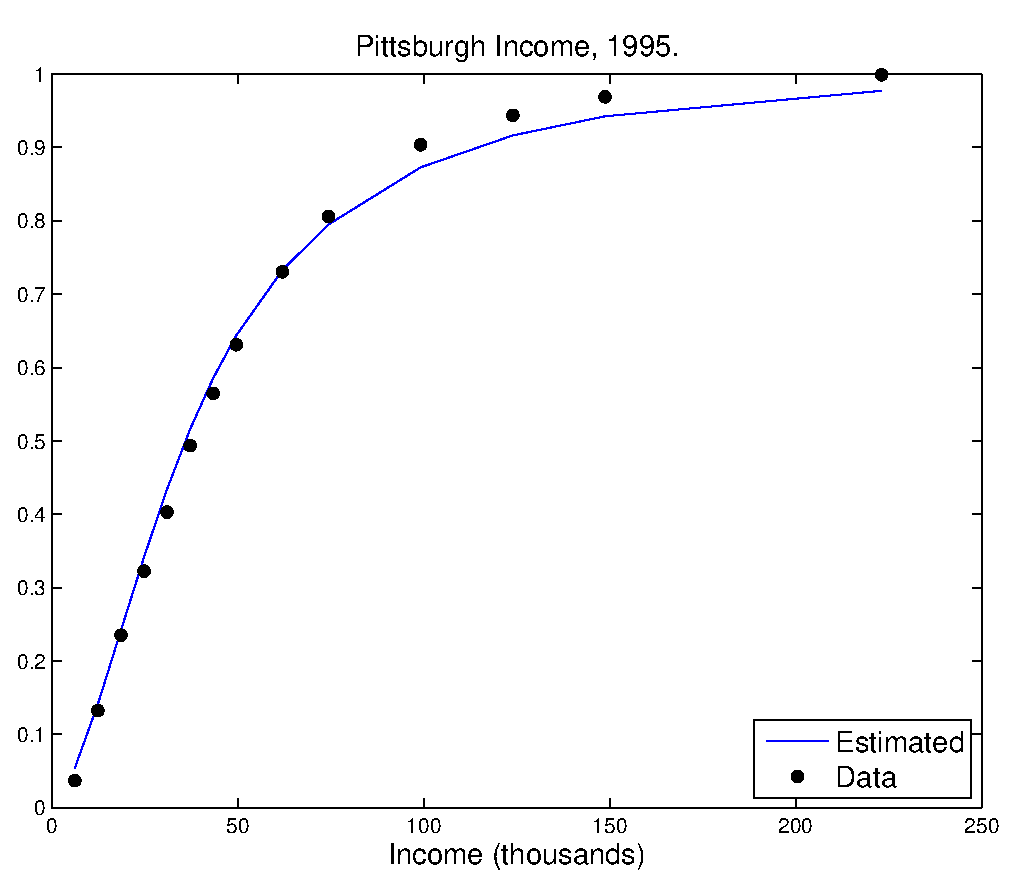
\includegraphics[width=\textwidth]{GLN4Fy.eps}
        \end{subfigure}%
        \begin{subfigure}[b]{0.5\textwidth}
                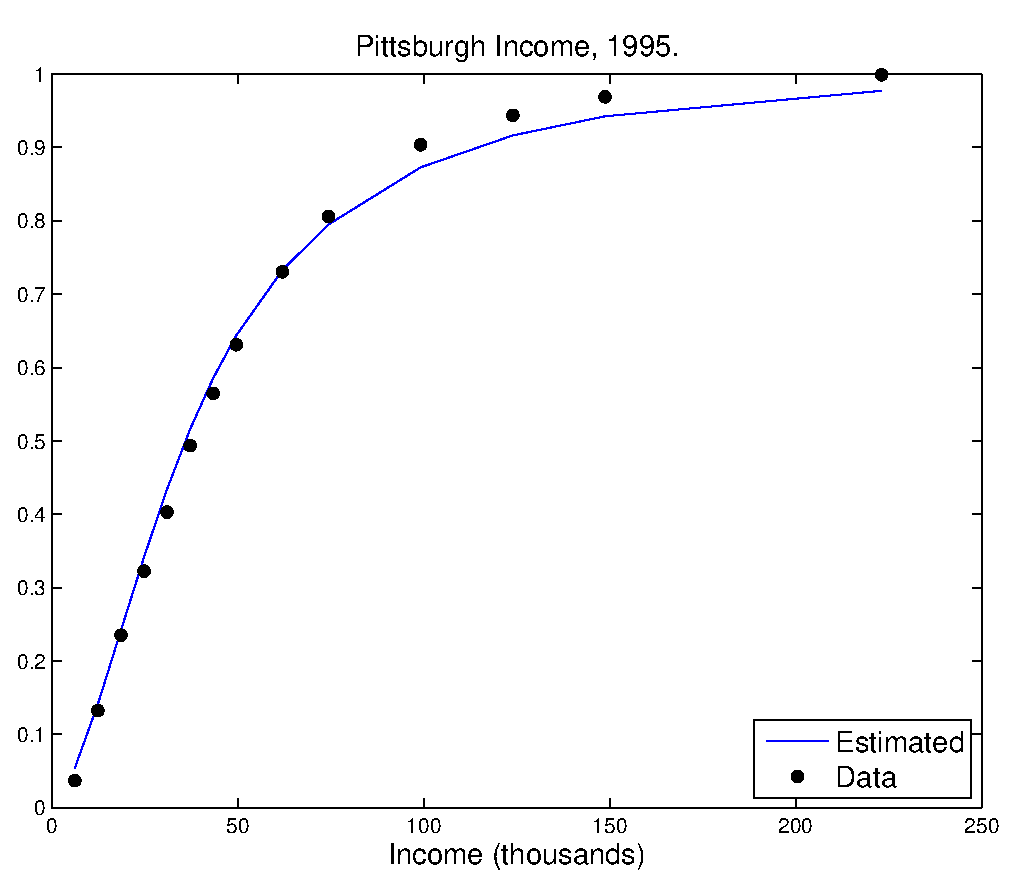
\includegraphics[width=\textwidth]{GLN4Fy.eps}
        \end{subfigure}
        \caption{Consumption Rule}
\end{figure}
}

\frame
{
  \frametitle{ The risk-free rate in heterogeneous-agent incomplete-insurance economies. Hugget (1993).}
Results 
\begin{figure}
        \begin{subfigure}[b]{0.5\textwidth}
                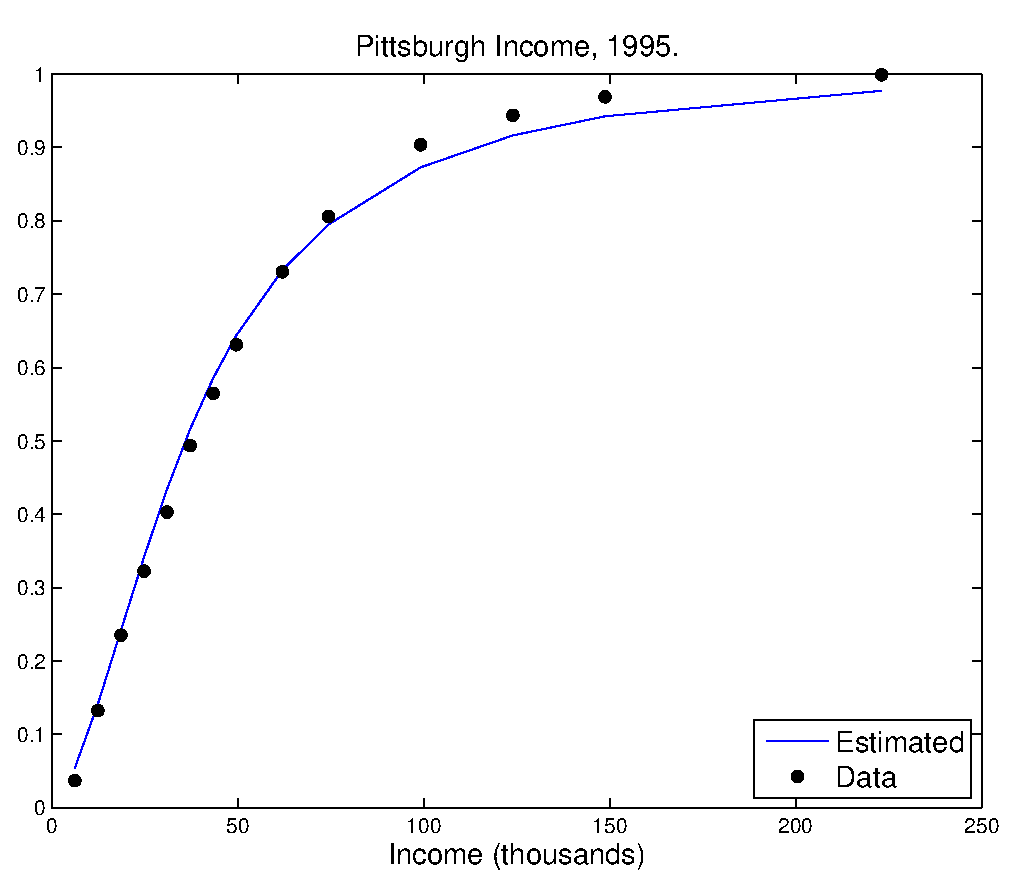
\includegraphics[width=\textwidth]{GLN4Fy.eps}
        \end{subfigure}%
        \begin{subfigure}[b]{0.5\textwidth}
                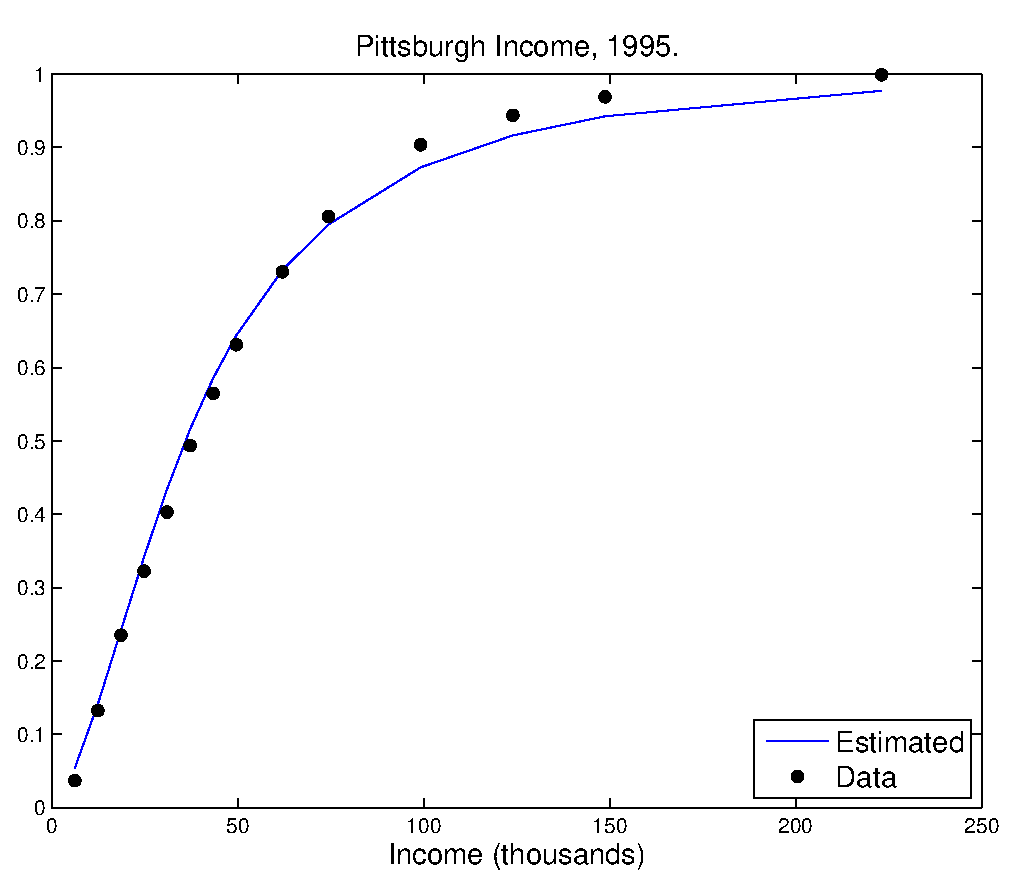
\includegraphics[width=\textwidth]{GLN4Fy.eps}
        \end{subfigure}
        \caption{Saving Rule}
\end{figure}
}

\frame
{
  \frametitle{ The risk-free rate in heterogeneous-agent incomplete-insurance economies. Hugget (1993).}
Results 
\begin{figure}
        \begin{subfigure}[b]{0.5\textwidth}
                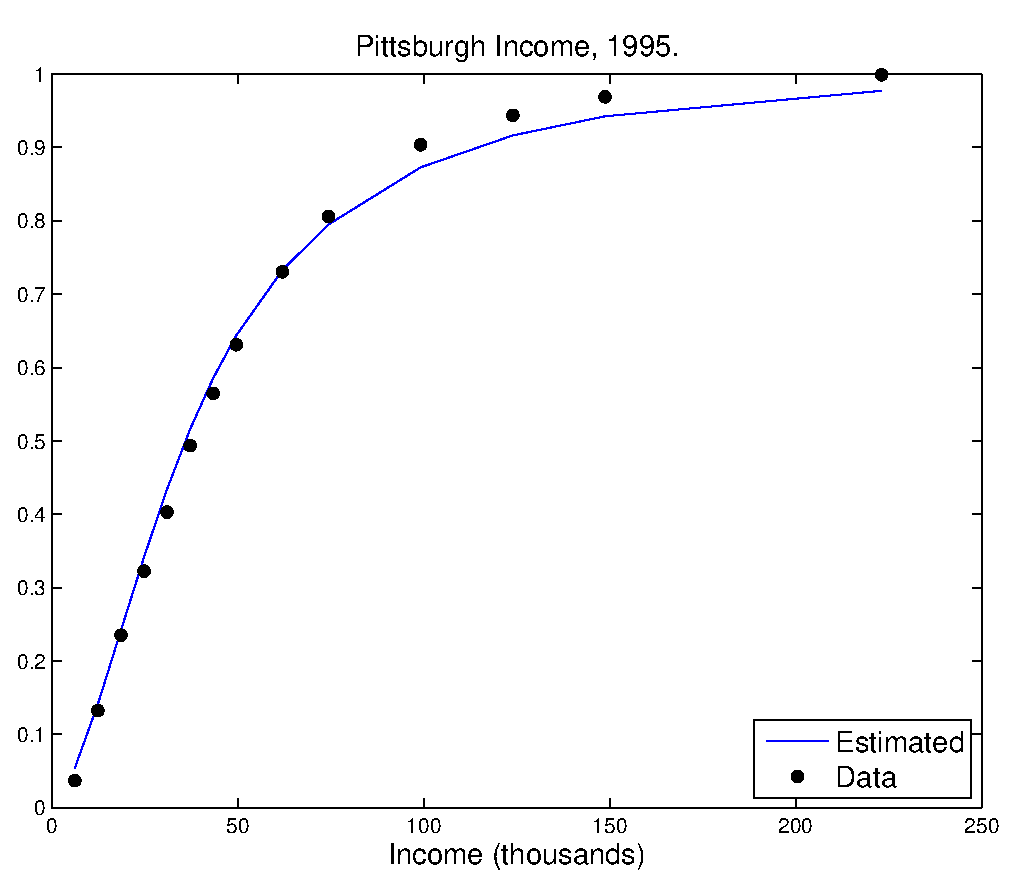
\includegraphics[width=\textwidth]{GLN4Fy.eps}
        \end{subfigure}%
        \begin{subfigure}[b]{0.5\textwidth}
                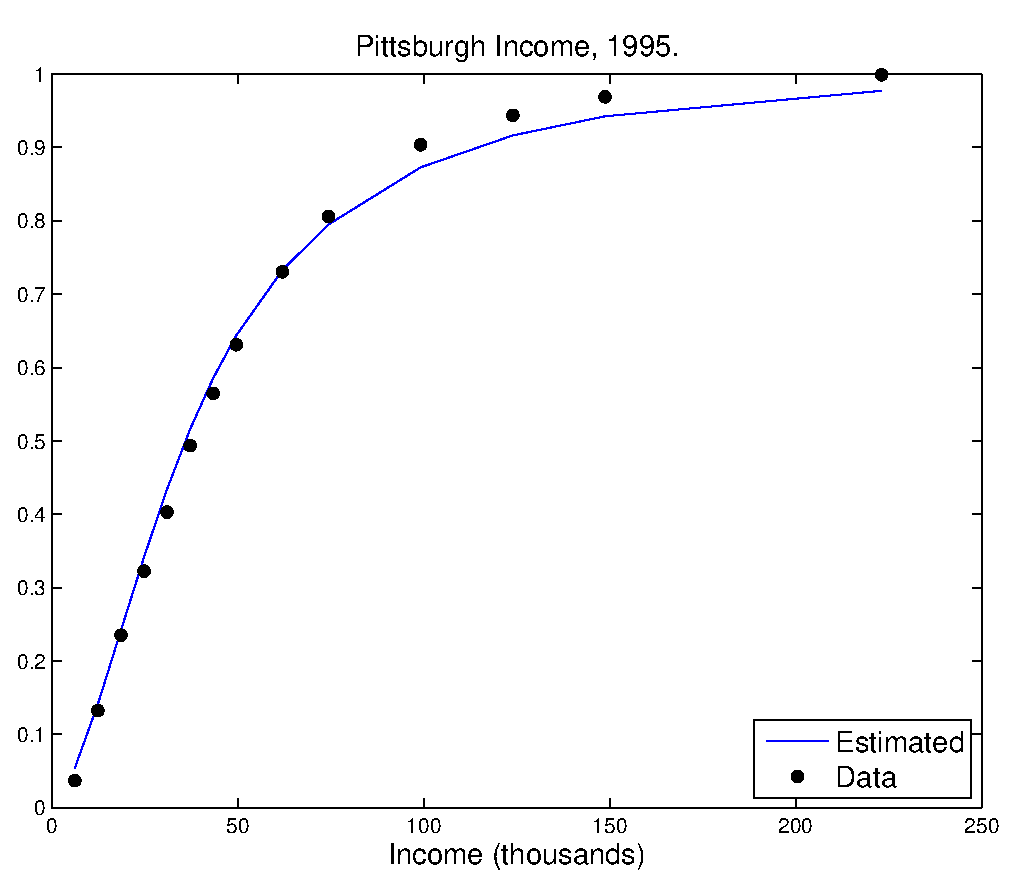
\includegraphics[width=\textwidth]{GLN4Fy.eps}
        \end{subfigure}
        \caption{Stationary Distribution}
\end{figure}
}


\frame
{
  \frametitle{ The risk-free rate in heterogeneous-agent incomplete-insurance economies. Hugget (1993).}
Comparative Statistics 
\begin{itemize}
\item Risk Aversion
\end{itemize}
}

\frame
{
  \frametitle{ The risk-free rate in heterogeneous-agent incomplete-insurance economies. Hugget (1993).}
Comparative Statistics 
\begin{itemize}
\item Borrowing Constraints
\end{itemize}
}


\end{document}